\begin{frame}{$k$-NN -- method summary}

% \maketag{Supervised} 
\maketag{regression} \maketag{classification}
\maketag{Nonparametric} \maketag[50]{White-box}

\medskip

\highlight{General idea}
\begin{itemize}
  \item \textbf{similarity} in feature space (w.r.t. certain \textbf{distance metric} $d(\xi,\xv)$) $\leadsto$ similarity in target space 
  % \item The \textbf{$k$-nearest neighbors ($k$-NN)} model is based on 
  % inter-observational \textbf{distances}, thus heavily depending on the chosen 
  % \textbf{distance measure}.
  \item \textbf{Prediction} for $\xv$: construct \textbf{$k$-neighborhood} 
  $N_k(\xv)$ from $k$ points closest to $\xv$ in $\Xspace$, then 
  predict
  \begin{itemize}
    \footnotesize
    \item (weighted) mean target for \textbf{regression}: 
    $\yh = \tfrac{1}{\sum\limits_{i: \xi \in N_k(\xv)} w_i}  
    \sum\limits_{i: \xi \in N_k(\xv)} w_i \yi $ with $w_i = \tfrac{1}{d(\xi,\xv)}$\\
    $\rightarrow$ optional: higher weights $w_i$ for close neighbors
    \item most frequent class for \textbf{classification}: 
    $\yh = \underset{\ell \in \gset}{\mathrm{\argmax}} \sum\limits_{i: \xi \in N_k(\xv)} \I(\yi = \ell)$\\
    $\Rightarrow$ Estimating posterior probabilities as $\hat{\pi}_{\ell}(\xi)= \frac{1}{k} \sum\limits_{i: \xi \in N_k(\xv)} \I(\yi = \ell)$
  \end{itemize}
  %\item No distributional or functional \textbf{assumptions}
  \item \textbf{Nonparametric} behavior: parameters = training data; no 
  compression of information
  \item Not immediately interpretable, but inspection of neighborhoods can be revealing
\end{itemize}
\end{frame}

% ------------------------------------------------------------------------------

\begin{frame}{$k$-NN -- method summary}

\medskip

\highlight{Hyperparameters} ~~ Neighborhood \textbf{size} $k$ (locality), 
\textbf{distance} metric (next page)

\vspace{5px}

\begin{minipage}{0.7\textwidth}
  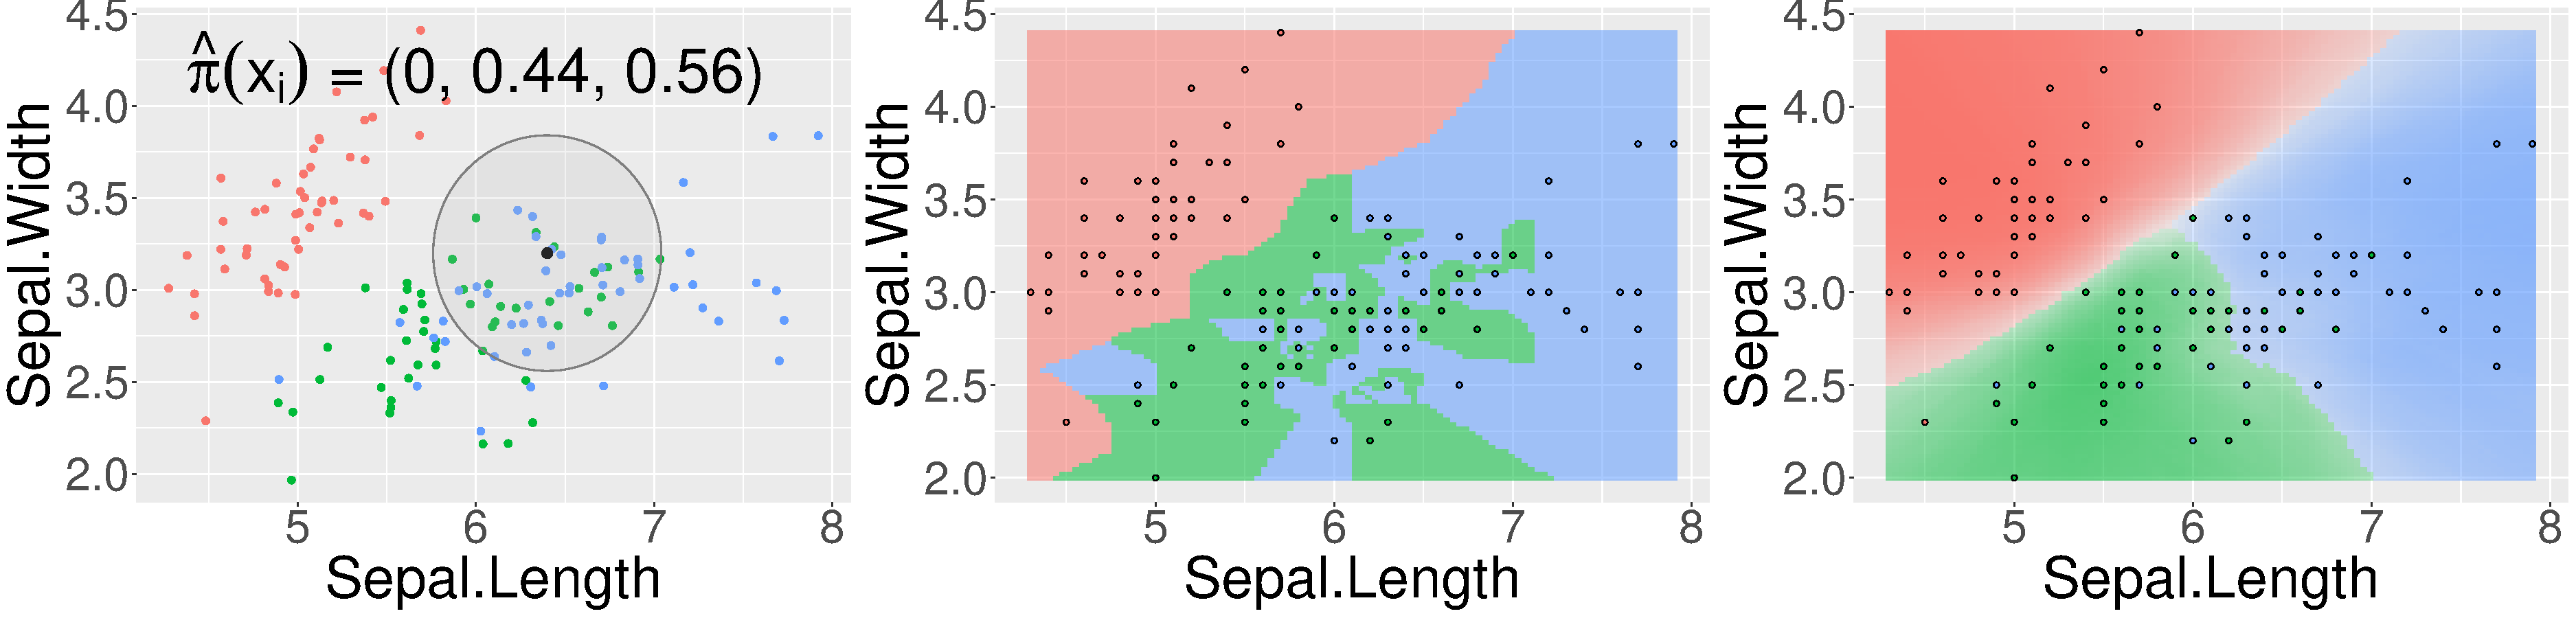
\includegraphics[width=\textwidth]{figure/knn-neighborhood.pdf}
\end{minipage}%
\hfill
\begin{minipage}{0.25\textwidth}
  \tiny
  \raggedright
  \textbf{Classification} \\
  \textit{Left}: Neighborhood for exemplary observation in \texttt{iris}, 
  $k = 50$ \\
  \textit{Middle}: Prediction surface for $k = 1$\\
  \textit{Right}: Prediction surface for $k = 50$
\end{minipage}

\begin{minipage}{0.7\textwidth}
\, \, \, 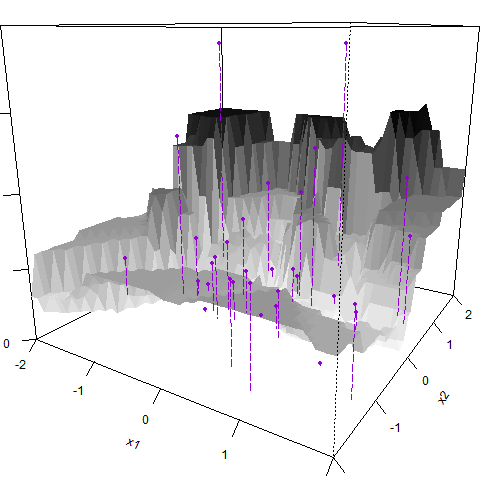
\includegraphics[width=0.3\textwidth]{figure/knn-reg-3d-3.png} \, \,
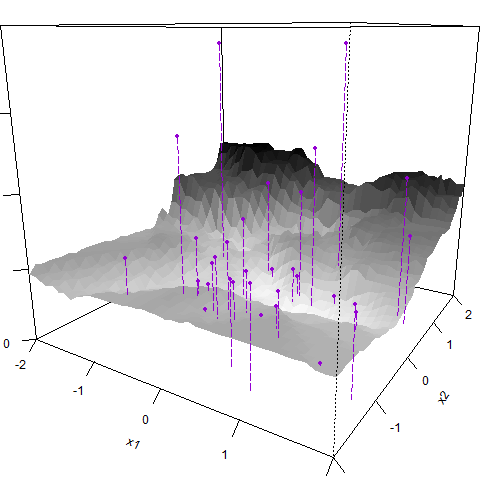
\includegraphics[width=0.3\textwidth]{figure/knn-reg-3d-7.png} \, \,
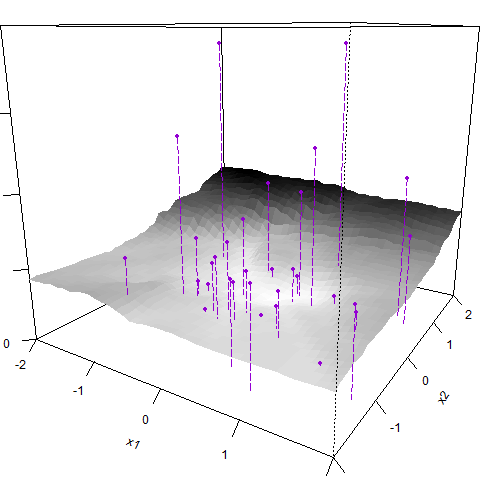
\includegraphics[width=0.3\textwidth]{figure/knn-reg-3d-15.png}
\end{minipage}%
\hfill
\begin{minipage}{0.25\textwidth}
  \tiny
  \raggedright
  \textbf{Regression} \\
  \textit{Left}: Prediction surface for $k = 3$\\ 
  \textit{Middle}: Prediction surface for $k = 7$\\
  \textit{Right}: Prediction surface for $k = 15$
\end{minipage}

\medskip

\begin{itemize}
    \item Small $k$ $\Rightarrow$ very local, "wiggly" decision boundaries
    \item Large $k$ $\Rightarrow$ rather global, smooth decision boundaries
\end{itemize}

\end{frame}

% ------------------------------------------------------------------------------

\begin{frame}{$k$-NN -- method summary}

\highlight{Popular distance metrics}

\begin{itemize}
  \item Numerical feature space:\\
  \begin{minipage}{0.7\textwidth}
  $\Rightarrow$ Typically, \textbf{Minkowski} distances
  $d(\xv, \xtil) = \|\xv - \xtil \|_q = 
  \left( \sum_j | x_j - \tilde{x_j} |^q
  \right)^{\tfrac{1}{q}}$
  \begin{itemize}
    \item $q = 1$: \textbf{Manhattan} distance $\rightarrow d(\xv, \xtil) =
    \sum_j | x_j - \tilde{x_j} |$
  \item $q = 2$: \textbf{Euclidean} distance $\rightarrow d(\xv, \xtil) =
  \sqrt{\sum_j (x_j - \tilde{x_j})^2}$
  \item Visualization: Manhatten (red, blue, yellow) vs. Euclidean (green)
  \end{itemize}
  %\item In presence of categorical features: \textbf{Gower} distance
\end{minipage}%
\begin{minipage}{0.25\textwidth}
 \begin{center}
  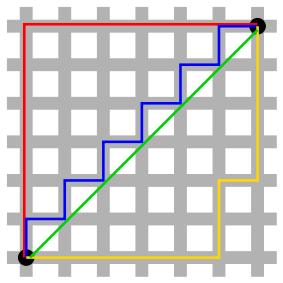
\includegraphics[width=.6\textwidth]{learners-overview/figure/manhattan_distance.png} %https://es.m.wikipedia.org/wiki/Archivo:Manhattan_distance.svg
 \end{center}
\end{minipage}
    \medskip
  \item Mixed feature space: 
  \begin{itemize}
%      \item Minkowski distances not applicable anymore
      \item \textbf{Gower distance} can handle numerical and categorical features, and missing data:\\ % (defined as \textit{similarity} by Gower, 1971):\\ %https://www.jstor.org/stable/2528823?seq=3#metadata_info_tab_contents
            - numerical: $d(x_i,x_j) =  \dfrac{|x_i-x_j|}{\max(x)-\min(x)}$\\
            - categorical: $d(x_i,x_j) =
            \begin{cases}
              1, \text{if\,} x_i \neq x_j\\
              0, \text{if\,} x_i = x_j
            \end{cases}$\\
            - Gower distance as average over individual scores
  \end{itemize}
  %\item \textbf{Custom} distance measures applicable
  \item Optional \textbf{weighting} to account for beliefs about varying feature
  importance
\end{itemize}
\vfill
  {\tiny Figure Source: \href{https://es.m.wikipedia.org/wiki/Archivo:Manhattan_distance.svg}{https://es.m.wikipedia.org/wiki/Archivo:Manhattan\_distance.svg}}
\end{frame}

% ------------------------------------------------------------------------------

\begin{frame}{$k$-NN -- Implementation \& Practical hints}

\footnotesize

\highlight{Preprocessing} ~~
Features should be standardized or normalized

\medskip

\highlight{Implementation}
\begin{itemize}
  \item \textbf{R:} \texttt{mlr3} learners (calling \texttt{kknn::kknn()})
  \begin{itemize}
    \item \textbf{Classification:}\\ 
    - \texttt{LearnerClassifKKNN}\\
    - \texttt{fnn::knn()}
    \item \textbf{Regression:}\\
    - \texttt{LearnerRegrKKNN}\\
    - \texttt{fnn::knn.reg()}
    \item Nearest Neighbour Search in $\order(N \log N)$: \texttt{RANN::nn2()}
  \end{itemize}
  \item \textbf{Python:} From package \texttt{sklearn.neighbors} 
  \begin{itemize}
    \item \textbf{Classification:}\\ 
    - \texttt{KNeighborsClassifier()}\\
    - \texttt{RadiusNeighborsClassifier()} as alternative if data not uniformly sampled
    \item \textbf{Regression:}\\
    - \texttt{KNeighborsRegressor()} \\
    - \texttt{RadiusNeighborsRegressor()} as alternative if data not uniformly sampled
  \end{itemize}
\end{itemize}

\end{frame}
% ------------------------------------------------------------------------------

\begin{frame}{$k$-NN -- Pros \& Cons}

\footnotesize

\begin{columns}[onlytextwidth]
  \begin{column}{0.5\textwidth}
    \highlight{Advantages}
    \footnotesize
    \begin{itemize}
      \positem Algorithm \textbf{easy} to explain and implement
      % \positem Applicable to both regression and classification
      \positem No distributional or functional \textbf{assumptions}\\
      $\rightarrow$ able to model data of \textbf{arbitrary complexity} %(in theory) 
      \positem No \textbf{training} or \textbf{optimization} required 
      %\positem Constant evolvement with \textbf{new data}
      \positem \textbf{local model} $\rightarrow$ \textbf{nonlinear} decision boundaries
      \positem Easy to \textbf{tune} (few hyperparameters)\\
      $\rightarrow$ number of neighbors $k$, distance metric
      % \positem Only one \textbf{hyperparameter} to tune
      \positem \textbf{Custom} distance metrics can often be easily designed to incorporate domain knowledge
    \end{itemize}
  \end{column}
  \begin{column}{0.5\textwidth}
    \highlight{Disadvantages}
    \footnotesize
    \begin{itemize}
      \negitem Sensitivity w.r.t. \textbf{noisy} or \textbf{irrelevant} features and outliers due to dependency on distance measure
      \negitem Heavily affected by \textbf{curse of dimensionality}
      \negitem Bad performance when feature \textbf{scales} are not consistent with feature relevance
      \negitem Poor handling of data \textbf{imbalances} (worse for more global model, i.e., large $k$)
      %\negitem High \textbf{memory} consumption of distance computation
    \end{itemize}
  \end{column}
\end{columns}

\end{frame}